\documentclass[12pt]{article}
\pdfoutput=1

\usepackage{scicite}
\usepackage{graphicx}
\usepackage{booktabs}
\usepackage{amsmath}
\usepackage[table,xcdraw]{xcolor}
\usepackage{times}
\usepackage{url}
\usepackage[normalem]{ulem}
\usepackage{comment}

\newif\ifdraft
\newif\iffinal
\newif\ifarxiv
\draftfalse
\finalfalse
\arxivtrue

\newcommand{\MBTODO}[2][]{\todo[color=blue!20,#1]{#2}}
\newcommand{\MJTODO}[2][]{\todo[color=orange!20,#1]{#2}}
\newcommand{\NBTODO}[2][]{\todo[color=green!40,#1]{#2}}


\ifarxiv % Include packages for appendix
\usepackage{caption}
\usepackage{subcaption}
\usepackage{textcomp}
\usepackage{array}
\usepackage{calc}
\usepackage{multirow}
\usepackage{mathtools}
\newcolumntype{L}[1]{>{\raggedright\let\newline\\\arraybackslash\hspace{0pt}}m{#1}}
\newcolumntype{C}[1]{>{\centering\let\newline\\\arraybackslash\hspace{0pt}}m{#1}}
\newcolumntype{R}[1]{>{\raggedleft\let\newline\\\arraybackslash\hspace{0pt}}m{#1}}
\newtheorem{lemma}{Lemma}
\newenvironment{proof}[1][Proof]{\textbf{#1.} }{\ \rule{0.5em}{0.5em}}
\fi

\ifdraft
\usepackage[textwidth=1.5in]{todonotes}
\usepackage[top=1.6in,bottom=1.1in,left=0.5in,right=1.7in]{geometry}
\else
\usepackage[disable]{todonotes}
\topmargin 0.0cm
\oddsidemargin 0.2cm
\textwidth 16cm 
\textheight 21cm
\footskip 1.0cm
\fi

\newenvironment{sciabstract}{%
\begin{quote} \bf}
{\end{quote}}

\iffinal
\renewcommand\refname{References and Notes}
\else
\fi

\iffalse
\newcounter{lastnote}
\newenvironment{scilastnote}{%
\setcounter{lastnote}{\value{enumiv}}%
\addtocounter{lastnote}{+1}%
\begin{list}%
{\arabic{lastnote}.}
{\setlength{\leftmargin}{.22in}}
{\setlength{\labelsep}{.5em}}}
{\end{list}}
\else
\newenvironment{scilastnote}{\paragraph{Acknowledgements.}}{}
\fi

\DeclareSymbolFont{extraup}{U}{zavm}{m}{n}
\DeclareMathSymbol{\heartsuit}{\mathalpha}{extraup}{86}
\DeclareMathSymbol{\diamondsuit}{\mathalpha}{extraup}{87}


\newcommand{\Qh}{{\sf Qh} }
\newcommand{\Kh}{{\sf Kh} }
\newcommand{\Jh}{{\sf Jh} }
\newcommand{\HUNL}{{HUNL}}
\newcommand{\HULH}{{HULHE}}
\newcommand{\CFRPlus}{{CFR$^{+}$}}
\newtheorem{theorem}{Theorem}
\allowdisplaybreaks 

\title{DeepStack: Expert-Level Artificial Intelligence in No-Limit Poker}

\author{
Matej Morav\v{c}\'{i}k$^{\spadesuit,\heartsuit,\dag}$, Martin Schmid$^{\spadesuit,\heartsuit,\dag}$, 
Neil Burch$^\spadesuit$, Viliam Lis\'y$^{\spadesuit,\clubsuit}$, \\
Dustin Morrill$^\spadesuit$, Nolan Bard$^\spadesuit$, Trevor Davis$^\spadesuit$, \\
Kevin Waugh$^\spadesuit$, Michael Johanson$^\spadesuit$, Michael Bowling$^{\spadesuit,\ast}$ \\
\normalsize{$^{\spadesuit}$Department of Computing Science, University of Alberta,}\\
\normalsize{Edmonton, Alberta, T6G2E8, Canada}\\
\normalsize{$^{\heartsuit}$Department of Applied Mathematics, Charles University,}\\
\normalsize{Prague, Czech Republic}\\
\normalsize{$^{\clubsuit}$Department of Computer Science, FEE, Czech Technical University,}\\
\normalsize{Prague, Czech Republic}\\
\\
\normalsize{$^\dag$These authors contributed equally to this work and are listed in alphabetical order.}
\\
\normalsize{$^\ast$To whom correspondence should be addressed; E-mail:  bowling@cs.ualberta.ca}
}

\date{}


%%%%%%%%%%%%%%%%% END OF PREAMBLE %%%%%%%%%%%%%%%%


\baselineskip24pt 

\begin{document} 
\maketitle 

\begin{sciabstract}
Artificial intelligence has seen a number of breakthroughs in recent years, with games often serving as significant milestones.  A common feature of games with these successes is that they involve information symmetry among the players, where all players have identical information.  This property of {\em perfect information}, though, is far more common in games than in real-world problems.  Poker is the quintessential game of {\em imperfect information}, and it has been a longstanding challenge problem in artificial intelligence.  In this paper we introduce DeepStack, a new algorithm for imperfect information settings such as poker. It combines recursive reasoning to handle information asymmetry, decomposition to focus computation on the relevant decision, and a form of intuition about arbitrary poker situations that is automatically learned from self-play games using deep learning.  In a study involving dozens of participants and 44,000 hands of poker, DeepStack becomes the first computer program to beat professional poker players in heads-up no-limit Texas hold'em.  Furthermore, we show this approach dramatically reduces worst-case exploitability compared to the abstraction paradigm that has been favored for over a decade.
\end{sciabstract}

Games have long served as a benchmark and set of milestones for progress in artificial intelligence.  
In the last two decades, we have seen computer programs reach a performance that exceeds expert human players in many games, e.g., backgammon~\cite{Tesauro95}, checkers~\cite{SchaefferEtAl96}, chess~\cite{CampbellEtAl02}, Jeopardy!~\cite{Ferucci12}, Atari video games~\cite{Mnih15:DQN}, and go~\cite{Silver16:AlphaGo}.
These successes all involve games with information symmetry, where all players have identical information about the current state of the game.
This property of {\em perfect information} is also at the heart of the algorithms that enabled these successes, e.g., local search during play~\cite{Samuel:AlphaBeta,Kocsis06:UCT}.

The founder of modern game theory and computing pioneer, von Neumann, envisioned reasoning in games without perfect information. ``Real life is not like that.  Real life consists of bluffing, of little tactics of deception, of asking yourself what is the other man going to think I mean to do.  And that is what games are about in my theory.''~\cite{Bronowski73}
One game that fascinated von Neumann was poker, where players are dealt private cards and take turns making bets or bluffing on holding the strongest hand, calling opponents' bets, or folding and giving up on the hand and the bets already added to the pot.
Poker is a game of {\em imperfect information}, where players' private cards give them asymmetric information about the state of game.

There has been some AI success in heads-up (i.e., two-player) {\em limit} Texas hold'em, the smallest variant of poker played by humans.\footnote{In 2008, Polaris defeated a team of professional poker players in heads-up limit Texas hold'em~\cite{Wired08}.  In 2015, Cepheus essentially solved the game~\cite{Bowling15:Cepheus}.}  However, heads-up limit Texas hold'em has fewer than $10^{14}$ decision points.  By comparison, computers have exceeded expert human performance in go~\cite{Silver16:AlphaGo}, a perfect information game with approximately $10^{170}$ decision points~\cite{allis1994}.  The comparable variant of poker is heads-up no-limit Texas hold'em (\HUNL).  In \HUNL, the two players can bet any number of chips, resulting in over $10^{160}$ decision points~\cite{Johanson13:Sizes}.  

Imperfect information games require more complex reasoning than their perfect information counterparts. 
The correct decision at a particular moment depends upon the probability distribution over private information that the opponent holds, which is revealed through their past actions.
However, how the opponent's actions reveal that information depends upon their knowledge of our private information and how our actions reveal it.
This kind of recursive reasoning is why one cannot easily reason about game situations in isolation, which is at the heart of local search methods for perfect information games.  
Competitive AI approaches in imperfect information games typically reason about the entire game and produce a complete strategy prior to play~\cite{ZinkevichEtAl07,GilpinEtAl07}.%
\footnote{%
End-game solving~\cite{Ganzfried15:Endgame,cprg:cfrd,Moravcik16:Subgames} is one exception to  computation occurring prior to play.  When the game nears the end, a new computation is invoked over the remainder of the game.  Thus, the program need not store this part of the strategy or can use a finer-grained abstraction aimed to improve the solution quality.  We discuss this as re-solving when we introduce DeepStack's new technique of \emph{continuous re-solving}.}
Counterfactual regret minimization (CFR)~\cite{ZinkevichEtAl07,cprg:cfrd,Bowling15:Cepheus} is one such technique that uses self-play to do recursive reasoning through adapting its strategy against itself over successive iterations.  If the game is too large to be solved directly, the common solution is to solve a smaller, abstracted game.  To play the original game, one {\em translates} situations and actions from the original game in to the abstract game.

While this approach makes it feasible for programs to reason in a game like \HUNL, it does so by squeezing \HUNL's $10^{160}$ situations into the order of $10^{14}$ abstract situations.  Likely as a result of this loss of information, such programs are well behind expert human play.  In 2015, the computer program Claudico lost to a team of professional poker players by a margin of 91 mbb/g,\footnote{We use milli-big-blinds per game (mbb/g) to measure performance in poker, where a milli-big-blind is one thousandth of the size of the big blind bet amount.  This normalizes performance for the number of games played and the size of stakes.  For comparison, a win rate of 50 mbb/g is considered a sizable margin by professional players and 750 mbb/g is the rate that would be lost if a player folded each game.\label{footnote:mbbh}}\ which is a ``huge margin of victory''~\cite{Wood15:PokerFuse-Claudico} and significant at a 90\% confidence level.  Furthermore, it has been recently shown that abstraction-based programs from the Annual Computer Poker Competition have massive flaws~\cite{Lisy16:LocalBR}. Four such programs (including top programs from the 2016 competition) were evaluated using a local best-response technique that produces an approximate lower-bound on how much a strategy can lose.  All four abstraction-based programs are beatable by over 3,000 mbb/g, which is four times as large as simply folding each game.

DeepStack takes a fundamentally different approach.  It continues to use the recursive reasoning of CFR to handle information asymmetry.  However, it does not compute and store a complete strategy prior to play and so has no need for explicit abstraction.  Instead it considers each particular situation as it arises during play, but not in isolation.  It avoids reasoning about the entire remainder of the game by substituting the computation beyond a certain depth with a fast approximate estimate.  This estimate can be thought of as DeepStack's intuition: a gut feeling of the value of holding any possible private cards in any possible poker situation.  Finally, DeepStack's intuition, much like human intuition, needs to be trained.  We train it with deep learning using examples generated from random poker situations.  We show that DeepStack is theoretically sound, produces substantially less exploitable strategies than abstraction-based techniques, and is the first program to beat professional poker players at \HUNL{} with a remarkable average win rate of over 450 mbb/g.

\section*{DeepStack}

DeepStack is a general-purpose algorithm for a large class of sequential imperfect information games.  For clarity, we will describe its operation in the game of \HUNL.  The state of a poker game
can be split into the players' private information, \emph{hands} of two cards dealt face down,
and the \emph{public state},
consisting of the cards laying face up on the table and the sequence
of betting actions made by the players. Possible sequences of public states in
the game form a \emph{public tree} with every public state having an associated \emph{public subtree}. 
See Figure~\ref{fig:public_tree}.

\begin{figure}[t]
\centering
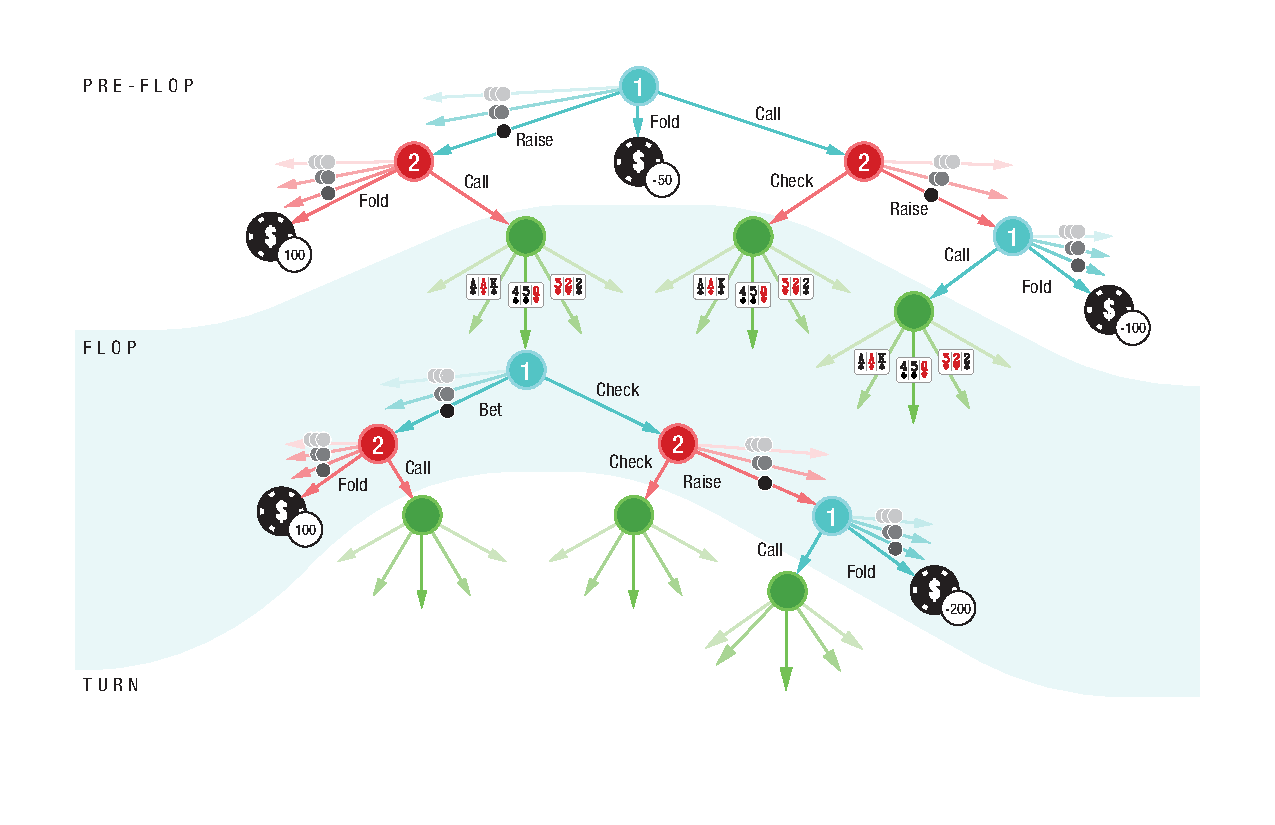
\includegraphics[width=0.8\textwidth]{figs/public_tree}
\caption{A portion of the public tree in \HUNL{}.  Red and turquoise edges represent player actions.  Green edges represent revealed public cards.  Leaf nodes with chips represent the end of the game, where the payoff may be fixed if a player folded or determined by the joint distribution of player hands given the preceding actions.}\label{fig:public_tree}
\end{figure}

A player's \emph{strategy} defines a probability distribution over
valid actions for each \emph{decision point}, which is a combination
of the public state and the hand for the acting player. Given a player's
strategy, for any public state one can compute the player's
\emph{range}, which is the probability distribution over the player's
possible hands given that the public state is reached.

Given both players' strategies, the \emph{expected utility} 
of a terminal public state, where the
game has ended, can be computed as a bilinear function of the players' ranges
using a payoff matrix determined by the rules of the game. The
expected utility of any other public state $s$, including the initial
state, 
is the expected utility over terminal states reached 
given the players'
strategies. A \emph{best response} strategy is one which
maximizes a player's expected utility against an opponent strategy.
In two-player, zero-sum games like \HUNL, a {\em solution} or
\emph{Nash equilibrium} strategy~\cite{Nash50:equilibrium} maximizes
the expected
utility when playing against a best response opponent strategy.
The \emph{exploitability} of a strategy is the difference in expected
utility against its best response opponent and the 
expected utility under a Nash equilibrium.  

The DeepStack algorithm seeks to compute and play a low-exploitability
strategy for the game, i.e., \emph{solve} for an approximate Nash equilibrium.
DeepStack computes this strategy during play\footnote{While DeepStack's strategy is computed 
during play, its strategy is static, albeit stochastic, since it is the result of a deterministic computation that produces a probability distribution over the available actions.}  
and only
for the states of the public tree that actually arise during play as illustrated in Figure~\ref{fig:deepstack-overview}.
This local
computation lets DeepStack reason in games that are too big for existing algorithms without having to abstract the
game's $10^{160}$ decision points down to $10^{14}$ to make solving tractable.
The DeepStack algorithm is composed of three ingredients: a sound local strategy computation for the current public state, depth-limited lookahead using a learned value function over arbitrary poker situations, and a restricted set of lookahead actions.  We explain each ingredient in turn, starting with the local lookahead procedure that by itself is computationally infeasible, before discussing the ingredients that make DeepStack tractable.

\begin{figure}[t]
\centering
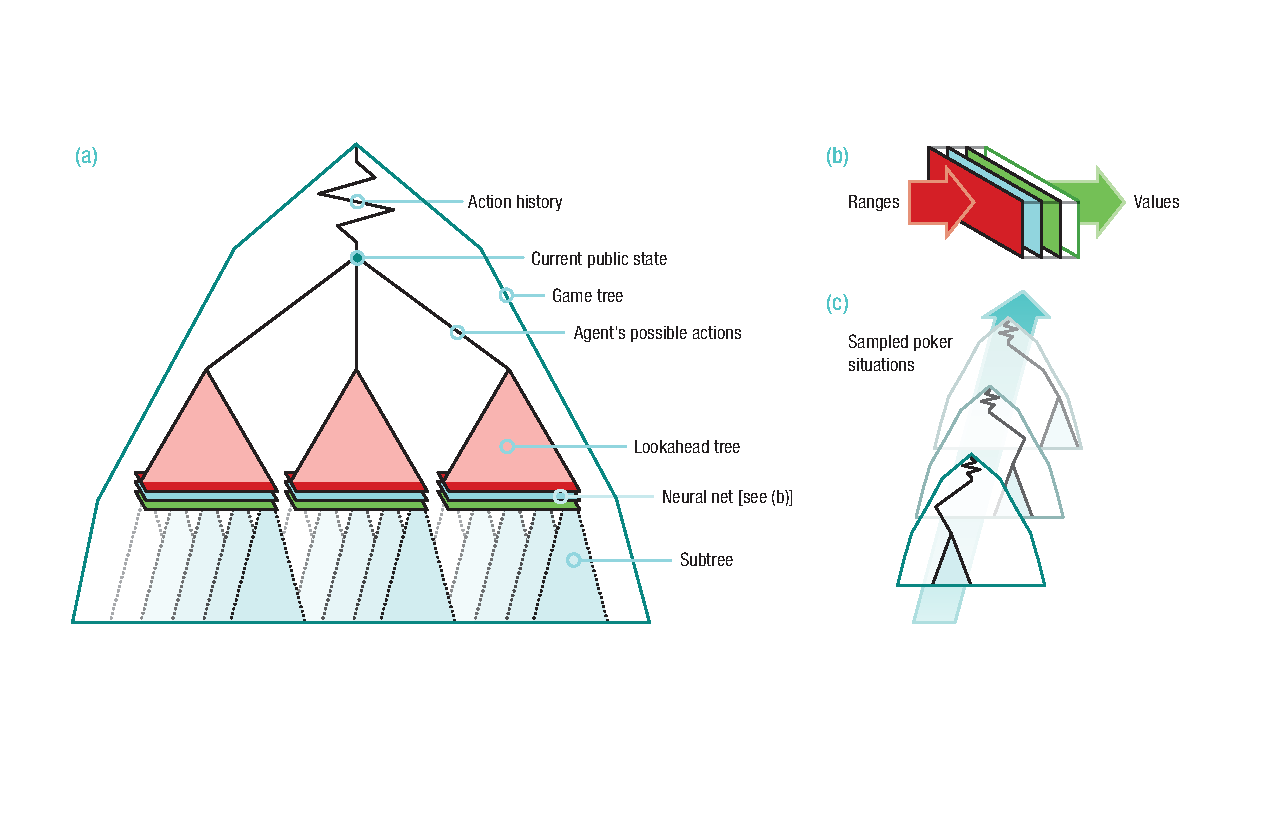
\includegraphics[width=0.7\textwidth]{figs/taking_actions}
\caption{DeepStack overview.  (a) DeepStack re-solves for its action at every public state it is to act, using a depth limited lookahead where subtree values are computed using a trained deep neural network (b) trained before play via randomly generated poker situations (c).}\label{fig:deepstack-overview}
\end{figure}

\subsection*{Continuous Re-Solving}
Suppose we have a solution for the entire game, 
but then in some public state we forget this strategy.  Can we reconstruct 
a solution for the subtree without having to solve the entire game again?
We can, through the process of \emph{re-solving}~\cite{cprg:cfrd}.  We need to know both our range at the public state and a vector of expected values achieved by the opponent under the previous solution for each opponent hand.  With these values, we can reconstruct a strategy for only the remainder of the game, which does not increase our overall exploitability.
Each value in the opponent's vector is a \emph{counterfactual
  value}, a conditional ``what-if'' value that gives the expected
value if the opponent reaches the public state with a particular hand.  The CFR algorithm also uses
counterfactual values, and if we use CFR as our solver, it is easy to compute the vector of opponent
counterfactual values at any public state.  

Re-solving, though, begins with a solution strategy, whereas our goal is to avoid ever maintaining a strategy for the entire game.  We get around this by doing \emph{continuous re-solving}: reconstructing a strategy by re-solving every time we need to act; never using the strategy beyond our next action.  To be able to re-solve at any public state, we need only keep track of our own range and a suitable vector of opponent counterfactual values.  These values must be an upper bound on the value the opponent can achieve with each hand in the current public state, while being no larger than the value the opponent could achieve had they deviated from reaching the public state.\footnote{This is an important relaxation of the counterfactual values used in re-solving, with a proof of sufficiency part of our proof of Theorem~\ref{thm} below~\cite{SOM}}

At the start of the game, our range is uniform and the opponent counterfactual values are initialized to the value of holding each private hand at the start.$^6$  When it is our turn to act we re-solve the subtree at the current public state using the stored range and opponent values, and act according to the computed strategy, discarding the strategy before we act again.  After each action --- our own, our opponent's, and chance --- we update our range and opponent counterfactual values according to the following rules:
\begin{itemize}
\item{\bf Own Action.}  Replace the opponent 
counterfactual values with those computed in the re-solved strategy for our chosen action.
Update our own range using the computed strategy and Bayes' rule.  
\item{\bf Chance Action.}  Replace the opponent counterfactual values with those computed for this chance action from the last re-solve.  Update our own range by zeroing hands in the range that are impossible given any new public cards.
\item{\bf Opponent Action.} Do nothing.
\end{itemize}
These updates ensure the opponent counterfactual values satisfy our sufficient conditions, and the whole procedure produces arbitrarily close approximations of a Nash equilibrium (see Theorem~\ref{thm}).
Notice that continuous re-solving never keeps track of the opponent's range, instead only keeping track of counterfactual values.  Furthermore, it never requires knowledge of the opponent's action to update these values, which is an important difference from traditional re-solving.  Both will prove key to making this algorithm efficient and avoiding any need for the translation step required with action abstraction methods~\cite{Gilpin08:Tartanian,Schnizlein09:Translation}.

\subsection*{Limited Lookahead and Sparse Trees}

Continuous re-solving is theoretically sound, but also impractical.  
While it does not ever maintain a complete strategy, re-solving itself is
intractable except near the end of the game. For example, re-solving for the first action would require temporarily computing an approximate solution for the whole game.  In order to make continuous re-solving practical, we need the second and third ingredients of DeepStack.  

\paragraph{Limited Depth Lookahead via Intuition.} 

When using CFR to solve or re-solve games, each player's strategy is improved locally on each iteration to smoothly approach a best-response.  In any public subtree(s), we could replace the iterative improvement with an explicit best-response.  Using explicit best-responses for both players means computing a Nash equilibrium strategy for these subtrees on each iteration.  This results in CFR-D~\cite{cprg:cfrd}, a game solving algorithm that saves space by not requiring subtree strategies (for example, in public states exceeding a fixed depth) to be stored.  However, it increases computation time by requiring the subtree strategies be recomputed on each iteration when only the vector of counterfactual values are needed.

Instead of solving subtrees to get the counterfactual values, DeepStack uses a learned value function intended to return an approximation of the values that would have been returned by solving. The inputs to this function
are the ranges for both players, the current pot size, and the public cards. 
The outputs are a vector for each player containing the counterfactual values of holding each hand in that situation.  In other words, the input is itself a description of a poker game: the probability distribution of being dealt individual private hands, the stakes of the game, and any public cards revealed; the output is an estimate of how valuable holding certain cards would be in such a game.  The value function is a sort of \emph{intuition}, a fast estimate of the value of finding oneself in an arbitrary poker situation.  Limiting the lookahead to depth four, and using a value function for all public states exceeding that depth, reduces the size of game for re-solving from $10^{160}$ decision points down to no more than $10^{17}$ decision points. DeepStack uses a deep neural network to approximate this function, which is described later.

A simpler form of using value functions to limit lookahead is at the heart of algorithms for perfect information games.  Deep Blue searched to a minimum depth of 12 moves on average, with some lines searching much deeper, before applying an evaluation function at positions beyond that depth~\cite{CampbellEtAl02}.  AlphaGo at shallow depths combined Monte Carlo rollout evaluations with the results of a trained evaluation function~\cite{Silver16:AlphaGo}.  In both cases the evaluation function needed to only return a single value given a single position in the game.  DeepStack's value function must be able to provide a vector of values given a probability distribution over positions in the game.

\paragraph{Sound Reasoning.}
DeepStack's depth-limited continuous re-solving is sound.  If DeepStack's intuition is ``good'' and ``enough'' computation is used in each re-solving step, then DeepStack plays an arbitrarily close approximation to a Nash equilibrium.
%
\begin{theorem}
If the values returned by the value function used when the depth limit is reached has error less than $\epsilon$, and $T$ iterations of CFR is used to re-solve, then the resulting strategy's exploitability is less than $k_1\epsilon + k_2 / \sqrt{T}$, where $k_1$ and $k_2$ are game-specific constants.\cite{SOM}
\label{thm}
\end{theorem}

\paragraph{Sparse Lookahead Trees.} 
 
The final ingredient in DeepStack is the reduction in the number of actions considered so as to construct a sparse lookahead tree.
DeepStack builds the lookahead tree using only the actions fold (if valid), 
call, 2 or 3 bet/raise actions, and all-in.  
While this step loses the soundness property of Theorem~\ref{thm} it moves DeepStack's re-solving time into the range of conventional human play.  With sparse and depth limited
lookahead trees, the re-solved games have approximately $10^{7}$ decision points, and can be solved 
in under five seconds.\footnote{We also use our sparse and depth limited lookahead computation to solve for the opponent's counterfactual values at the start of the game, which are used to initialize DeepStack's continuous re-solving.\label{footnote:start-values}}

While this ingredient looks very similar to action abstraction~\cite{Gilpin08:Tartanian,Schnizlein09:Translation}, which often results in highly exploitable strategies~\cite{Lisy16:LocalBR}, there are important distinctions.  Each re-solve in DeepStack starts from the actual public state and so always knows the exact size of the pot.  Second, the algorithm never uses the opponent's actual action to update its range or the opponent counterfactual values, and so no translation of opponent bets are ever needed.  
%Finally, while it is known that not all actions are necessary in a solution~\cite{Schmid14:Bounding}, we have observed empirically that our further reduced set of actions doesn't change the counterfactual values much, even while the strategies themselves vary wildly~\cite{SOM}.

\section*{Deep Counterfactual Value Networks}

Deep neural networks (DNNs) have proven to be powerful models and are responsible for major advances in image and speech recognition\cite{Krizhevsky12:ImageNet,Hinton12:Speech}, automated generation of music \cite{Oord16:WaveNet}, and game-playing~\cite{Mnih15:DQN,Silver16:AlphaGo}.
DeepStack uses DNNs, with a tailor-made architecture, as the value function for its depth-limited lookahead.
See Figure~\ref{fig:dnn}.  Two separate networks are trained: one estimates the counterfactual values after the first three public cards are dealt (flop network), the other after dealing the fourth public card (turn network). An auxiliary network for values before any public cards are dealt is used to speed up the re-solving for early actions~\cite{SOM}.

\paragraph{Architecture.}  DeepStack uses a standard feed-forward network with seven fully connected hidden layers each with 500 nodes and parametric rectified linear units~\cite{He15:PReLU} for the output.  This basic architecture is embedded in an outer network that guarantees the counterfactual values satisfy the zero-sum property.  The outer computation takes the estimated counterfactual values, and computes a weighted sum using the two players' input ranges resulting in separate estimates of the game value.  These two values should sum to zero, but may not.  Half the actual sum is then subtracted from the two players' estimated counterfactual values.  
This entire computation is differentiable and can be trained with gradient descent.  The network's inputs are the pot-size as a fraction of the players' total stacks and an encoding of the players' ranges as a function of the public cards.  The ranges are encoded by bucketing hands, as in traditional abstraction methods~\cite{Shi00:Rhode,Gilpin07:Abstraction,Johanson13:Abstraction}, and input as a vector of probabilities over the buckets.  Note that while this bucketing results in some loss of information, it is only used to estimate counterfactual values at the end of a lookahead tree rather than limiting what information the player has about their cards when acting. 
The output of the network are vectors of counterfactual values for each player and hand, interpreted as fractions of the pot size.

\begin{figure}[t]
\centering
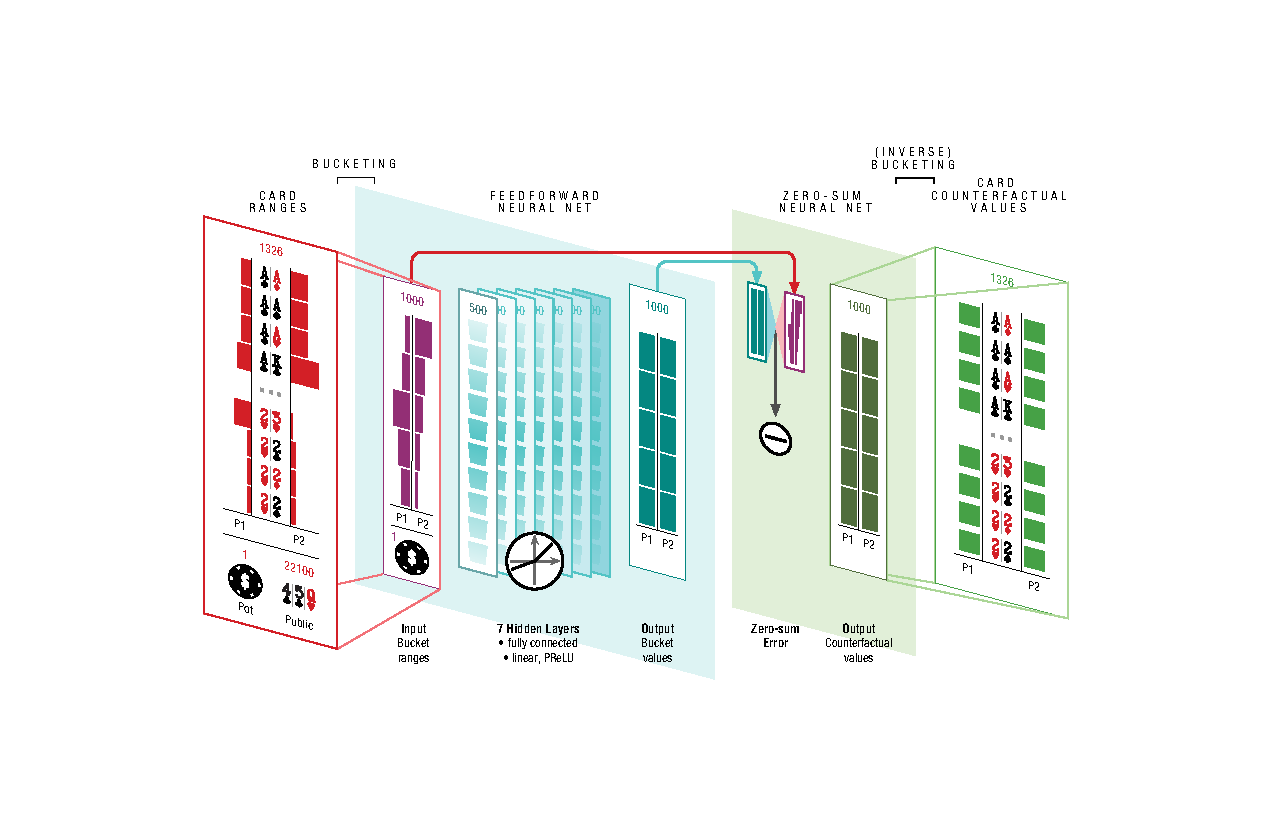
\includegraphics[width=0.8\textwidth]{figs/dnn}
\caption{Deep counterfactual value networks.  The inputs to the network are the pot size, public cards, and the player ranges, which are first processed into bucket ranges.  The output from the seven fully connected hidden layers is post-processed to guarantee the values satisfy the zero-sum constraint, and then mapped back into hand counterfactual values. }\label{fig:dnn}
\end{figure}

\paragraph{Training.}  The turn network was trained by solving 10 million randomly generated poker \emph{turn games}.  These turn games used randomly generated ranges~\cite{SOM}, public cards, and a random pot size.  The target counterfactual values for each training game were generated by solving the game with players' actions restricted to fold, call, a pot-sized bet, and an all-in bet, but no card abstraction.  The flop network was trained similarly with 1 million randomly generated \emph{flop games}.  However, the target counterfactual values were computed using our limited-depth solving procedure and our trained turn network.  The networks were trained using the Adam gradient descent optimization procedure\cite{kingma2014adam} with a Huber loss \cite{huber1964}. 

\section*{Evaluating DeepStack}

We evaluated DeepStack by playing it against a pool of professional poker players recruited by the International Federation of Poker\cite{IFP}.  Thirty-three players from 17 countries were recruited.  Each was asked to complete a 3,000 game match over a period of four weeks between November 7th and December 12, 2016.  Cash incentives were given to the top three performers (\$5,000, \$2,500, and \$1,250 CAD).  

Evaluating performance in \HUNL{} is challenging because of the large variance in per-game outcomes due to randomly dealt private and public cards and stochastic choices made by the players.  The better player may lose in a short match simply because they were dealt weaker hands or their rare bluffs were made at inopportune times.  As seen in the Claudico match~\cite{Wood15:PokerFuse-Claudico}, even 80,000 games may not be enough to statistically significantly separate players whose skill differs by a considerable margin.  We evaluate performance using AIVAT~\cite{Burch16:AIVAT}, a provably unbiased low-variance technique for evaluating performance in imperfect information games based on carefully constructed control variates.  AIVAT requires an estimated value of holding each hand in each public state, and then uses the expected value changes that occur due to chance events and actions of players with known strategies to compute its control variate.  DeepStack's own value function estimate is perfectly suited for AIVAT.  And indeed when used with AIVAT we get an unbiased performance estimate with an impressive $85\%$ reduction in standard deviation.  Thanks to this technique, we can show statistical significance in matches with as few as 3,000 games.

\begin{figure}[t]
\centering
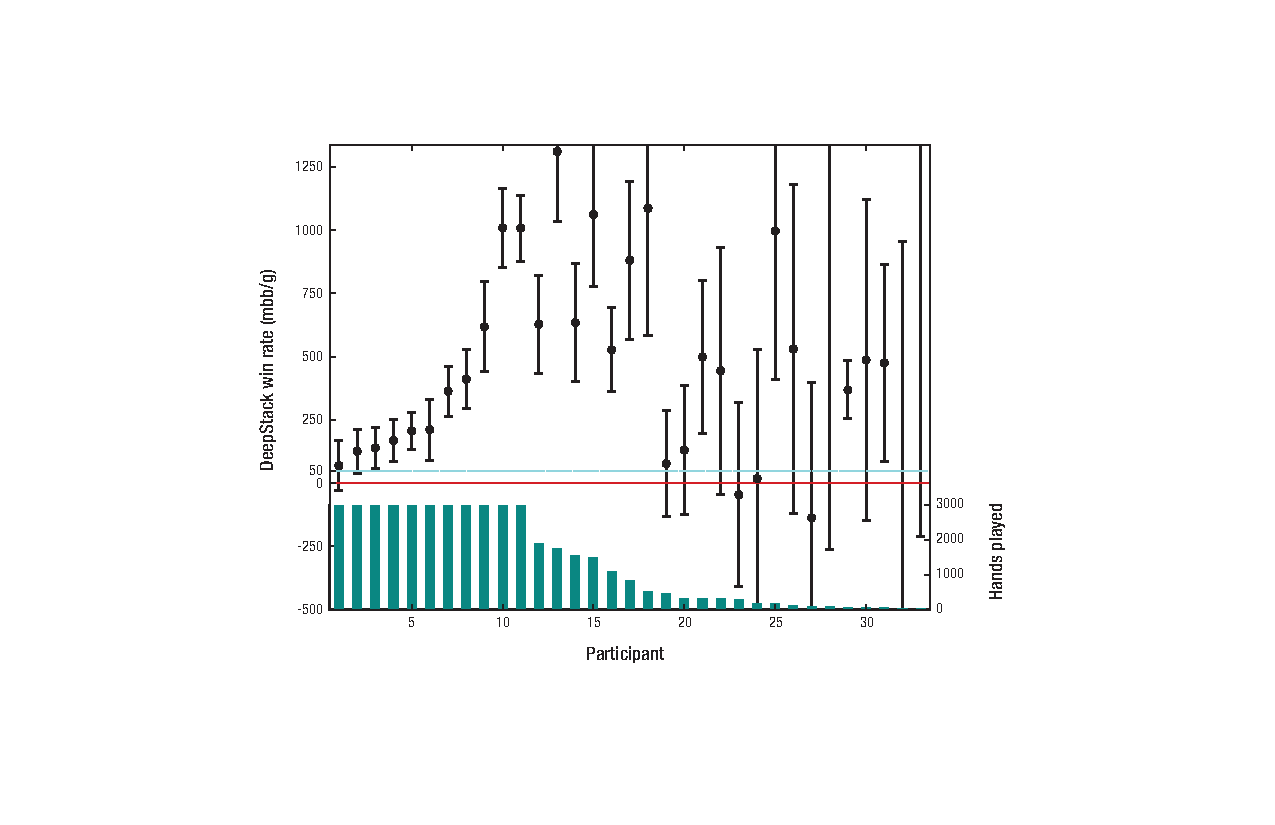
\includegraphics[width=0.7\textwidth]{figs/humans_curio}
\caption{Performance of professional poker players against DeepStack estimated with AIVAT along with a 95\% confidence interval. The solid bars at the bottom show the number of games the participant completed.}\label{fig:humans}
\end{figure}

In total 44,852 games were played by the thirty-three players with 11 players completing the requested 3,000 games.
Over all games played, DeepStack won 492 mbb/g.  This is over 4 standard deviations away from zero, and so highly significant.  Note that professional poker players consider 50 mbb/g a sizable margin.  Using AIVAT to evaluate performance, we see DeepStack was overall a bit lucky, with its estimated performance actually 486 mbb/g.  However, as a lower variance estimate, this margin is over 20 standard deviations from zero, and so we are certain to be outperforming our pool of professional players.  

The performance of individual participants measured with AIVAT is summarized in Figure~\ref{fig:humans}.
Amongst those players that completed the full 3,000 games, DeepStack is estimated to be winning by 394 mbb/g, and individually beating 10 out of 11 such players by a statistically significant margin.  Only for the top player, still estimated to be losing by 70 mbb/g, is the result not a statistically significant margin.
More details on the participants and their results are presented in the supplemental material~\cite{SOM}.

\subsection*{Exploitability}

The main goal of DeepStack is to approximate Nash equilibrium play, i.e., minimize exploitability.
While the exact exploitability of a \HUNL{} poker strategy is intractable to compute, the recent local best-response technique (LBR) can provide a lower bound on a strategy's exploitability~\cite{Lisy16:LocalBR} given full access to its action probabilities.  LBR uses the action probabilities to compute the strategy's range at any public state.  Using this range it chooses its response action from a fixed set using the  assumption that no more bets will be placed for the remainder of the game.  Thus it best-responds locally to the opponent's actions, providing a lower-bound on their overall exploitability.  As already noted, abstraction-based programs from the Annual Computer Poker Competition are highly exploitable by LBR: four times more exploitable than folding every game.  However, even under a variety of settings, LBR fails to exploit DeepStack at all --- itself losing by over 350 mbb/g to DeepStack~\cite{SOM}.  Either a more sophisticated lookahead is required to identify its weaknesses or DeepStack is substantially less exploitable. 

\section*{Discussion}

DeepStack is the first computer program to defeat professional poker players at heads-up no-limit Texas Hold'em, an imperfect information game with $10^{160}$ decision points.  Notably it achieves this goal with almost no domain knowledge or training from expert human games.  The implications go beyond just being a significant milestone for artificial intelligence.  DeepStack is a paradigmatic shift in approximating solutions to large, sequential imperfect information games.  
Abstraction and offline computation of complete strategies has been the dominant approach for almost 20 years~\cite{Shi00:Rhode,BillingsEtAl03,Sandholm12}.  
DeepStack allows computation to be focused on specific situations that arise when making decisions and the use of automatically trained value functions.  These are two of the core principles that have powered successes in perfect information games, albeit conceptually simpler to implement in those settings.  As a result, for the first time the gap between the largest perfect and imperfect information games to have been mastered is mostly closed.

As ``real life consists of bluffing... deception... asking yourself what is the other man going to think''~\cite{Bronowski73}, DeepStack also has implications for seeing powerful AI applied more in settings that do not fit the perfect information assumption.  The old paradigm for handling imperfect information has shown promise in applications like defending strategic resources~\cite{Lisy16:cfr-security} and robust decision making as needed for medical treatment recommendations~\cite{ChenBowling12}.  The new paradigm will hopefully open up many more possibilities.

\bibliography{paper}
\bibliographystyle{Science}

\begin{scilastnote}
We would like to thank IFP, all of the professional players who committed valuable time to play against DeepStack, and
R.~Holte, A.~Brown, and K.~Bla\v{z}kov\'a for comments on early drafts of this article.
We especially would like to thank IBM, from which the two first authors are on leave (IBM Prague), for their support of this research through an IBM faculty grant.  
The research was also supported by Alberta Innovates through the Alberta Machine Intelligence Institute, the Natural Sciences and Engineering Research Council of Canada, and Charles University (GAUK) Grant no. 391715.  
This work was only possible thanks to computing resources provided by Compute Canada and Calcul Qu\'ebec.  
\end{scilastnote}

\ifarxiv
\clearpage
\begin{center}
{\LARGE\baselineskip24pt 
Supplementary Materials for \\
{\large DeepStack: Expert-Level AI in No-Limit Poker}
\par\bigskip\bigskip\bigskip
}
\end{center}

\input{appendix}
\fi

\end{document}
